\documentclass{article}

\usepackage[nonatbib,preprint]{neurips_2024}

\usepackage[utf8]{inputenc}
\usepackage[T1]{fontenc}
\usepackage{hyperref}
\usepackage{url}
\usepackage{booktabs}
\usepackage{amsfonts}
\usepackage{nicefrac}
\usepackage{microtype}
\usepackage{xcolor}
\usepackage{amsmath}
\usepackage{graphicx}
\graphicspath{{figs/}}

\title{Random Features, Kernel Approximation, and Double Descent\\on Tabular Regression}

\author{%
 Nicholas Welsh \\
  Department of Computer Science\\
  Department of Mathematics \\
  Florida Institute of Technology\\
  Melbourne, FL 32901 \\
  \texttt{nwelsh2024@my.fit.edu}
}

\begin{document}
\maketitle

\begin{abstract}
The classical bias-variance tradeoff predicts that test error rises monotonically once a model has more parameters than training points. The double-descent phenomenon (Belkin et al., 2019) contradicts that prediction, showing a spike near the interpolation threshold $P = N$ followed by a second descent. This project reproduces the spike on California Housing using random Fourier feature ridge regression and tests the three-factor explanation of Schaeffer et al.\ (2023) by ablating each factor in turn. Ridge regularization, leading-singular-direction projection, and noiseless targets each eliminate the spike on their own, with ridge $\lambda = 0.1$ collapsing test MSE at the threshold from $\sim 2 \times 10^4$ to $0.31$. The smallest singular value of the random feature matrix drops to $6 \times 10^{-7}$ at $P = N$ and recovers in the overparameterized regime, supporting the geometric explanation of the spike. Random-feature ridge also approaches exact RBF kernel ridge as $P \to \infty$, recovering the Rahimi and Recht (2007) kernel-approximation result on the same pipeline.
\end{abstract}

\section{Introduction}

The classical bias-variance tradeoff teaches that increasing model capacity beyond the interpolation threshold should overfit. Modern practice routinely produces overparameterized models that generalize well, with double-descent test-error curves (Belkin et al., 2019) showing a spike at the interpolation threshold $P \approx N$ and a second descent past it. Throughout this report, $N$ is the training-set size and $P$ is the number of random features. The interpolation threshold is the regime where the model has just enough parameters to fit the training data exactly.

Double descent is surprising because classical bias-variance theory predicts only one thing past the interpolation threshold, namely monotonic overfitting, while practice shows a sharp test-error spike followed by a second descent. The phenomenon was widely observed in deep-learning practice for years before Belkin et al.\ (2019) made it a named effect with a clean empirical demonstration. Schaeffer et al.\ (2023) sharpen the question by isolating three factors that jointly produce the spike, each of which can be ablated independently. That gives a concrete experimental program where each factor predicts a separate cure that can be tested in isolation, which is exactly what the rest of this report does.

The central question this project asks is concrete.

\begin{center}
\emph{Where does the classical curve break, and what fixes it?}
\end{center}

Schaeffer et al.\ (2023) argue that the spike is driven by three factors that act in concert. Factor (a) is the smallest singular value of the feature matrix vanishing as $P \to N$. Factor (b) is test-feature variation concentrated in the trailing singular directions, which amplifies (a). Factor (c) is the presence of target residuals that are not in the column space of the training features, which is what (a) and (b) ultimately amplify. Removing any one factor flattens the spike.

We reproduce the double-descent curve with random Fourier features on a tabular regression task (California Housing) and test the three-factor explanation by ablating each factor in turn. The same random-feature pipeline approximates the exact RBF kernel ridge regressor as $P \to \infty$, recovering the Rahimi and Recht (2007) kernel-approximation reference point on the same code.

\subsection{Contributions}
\begin{itemize}
  \item \textbf{Reproduction of double descent on California Housing.} Test MSE peaks at $P \approx 300$ ($N = 256$) at $1.21$ and descends to $0.75$ in the overparameterized regime ($P = 4096$).
  \item \textbf{Three-factor ablation.} At $P = N$, increasing ridge regularization from $\lambda = 0$ to $\lambda = 0.1$ reduces test MSE from $\sim 2 \times 10^4$ (numerical-instability blowup) to $0.31$. Projecting test features onto the top-$N/4$ singular directions of the training feature matrix reduces test MSE to $0.35$. Replacing the targets with the best linear fit reduces test MSE from the same blowup to $1.33$. Each factor alone eliminates the spike.
  \item \textbf{Spectral collapse at the interpolation threshold.} The smallest singular value of the random-feature matrix drops from $0.082$ at $P = 64$ to $6 \times 10^{-7}$ at $P = N$, then rises again to $\sim 0.003$ for $P \gg N$. The dip is exactly at the interpolation threshold and matches the location of the test-error spike.
  \item \textbf{Kernel approximation.} Random-feature ridge converges to a region near the exact RBF kernel ridge baseline as $P$ grows, although on California Housing the linear ridge baseline outperforms the RBF kernel for the chosen bandwidth, and we discuss this honestly in the limitations.
\end{itemize}

\section{Related Work}

\paragraph{Random features.}
Rahimi and Recht (2007) introduced random Fourier features as a stochastic approximation to translation-invariant kernels. The construction samples random frequencies $\omega_i \sim \mathcal{N}(0, \sigma^{-2} I)$ and phases $b_i \sim \mathrm{Unif}(0, 2\pi)$, and the map $\phi(x)_i = \sqrt{2/P}\, \cos(\omega_i^\top x + b_i)$ produces a feature embedding whose inner product approximates the RBF kernel as $P$ grows.

\paragraph{Double descent.}
Belkin et al.\ (2019) documented the phenomenon empirically across linear models, decision trees, and neural networks. Many subsequent papers have studied its mechanism in linear and random-feature regression (Hastie et al., 2022, Bartlett et al., 2020, Mei and Montanari, 2022). The geometry-driven account in Schaeffer et al.\ (2023) identifies three factors that jointly produce the spike, with each factor sufficient to remove it.

\paragraph{Kernel ridge regression and kernel PCA.}
Exact RBF kernel ridge regression solves $\hat{\alpha} = (K + \lambda I)^{-1} y$ on the training kernel matrix and predicts $\hat{y}_{\text{test}} = K_{\text{test}, \text{train}} \hat{\alpha}$ (Rasmussen and Williams, 2006). Kernel PCA (Sch\"olkopf, Smola, and M\"uller, 1998) provides an unsupervised view of the same kernel through its singular spectrum.

\section{Data and Setup}

\paragraph{Why tabular.}
Random-feature ridge regression is the cleanest setting for studying double descent. Image and text data introduce architecture-specific confounds (convolutional inductive biases, attention patterns) that mask the pure feature-and-regression dynamics that the three-factor account predicts. Tabular regression isolates exactly the behavior under study.

\paragraph{Dataset.}
California Housing (Pace and Barry, 1997) provides $20\,640$ rows with 8 numeric features and a continuous target. We load it through scikit-learn's built-in loader. We hold out $20\%$ of the rows as a fixed test set ($N_{\text{test}} = 4128$) and take a small training subset of $N = 256$ rows from the remaining $80\%$. Both features and target are standardized using statistics from the training subset only. Holding $N$ small makes the interpolation threshold $P = N$ cheap to span.

\paragraph{Random Fourier features.}
We use the cosine variant from Rahimi and Recht (2007), $\phi(x)_i = \sqrt{2/P}\, \cos(\omega_i^\top x + b_i)$ with $\omega_i \sim \mathcal{N}(0, \sigma^{-2} I_d)$ and $b_i \sim \mathrm{Unif}(0, 2\pi)$. The "cosine" name distinguishes this from the sin/cos paired version, where each random direction contributes two features (a sine and a cosine) instead of one. The cosine variant uses one cosine feature per direction with a uniform random phase. Bandwidth $\sigma = 2.279$ is set by the median pairwise-distance heuristic on the training subset.

\paragraph{Sweep configuration.}
We sweep
\[
P \in \{4, 8, 16, 32, 64, 128, 200, 240, 256, 272, 300, 350, 512, 1024, 2048, 4096\},
\]
with three random-feature seeds per $P$. For each $P$, we fit ridge regression with $\lambda = 10^{-3}$ as the default. We use the closed-form solution. In the underparameterized regime $P < N$ we solve $(\Phi^\top \Phi + \lambda I) w = \Phi^\top y$. In the overparameterized regime $P \geq N$ we use the dual form $w = \Phi^\top (\Phi \Phi^\top + \lambda I)^{-1} y$ for numerical stability.

\paragraph{Headline metric.}
We report mean squared error (MSE) on the test holdout, averaged over three random-feature seeds. Lower is better. All MSE values are reported on standardized targets (zero mean and unit variance on the training subset), so a mean predictor scores around $0.84$ and a perfect predictor would score $0.00$.

\section{Methods}

\paragraph{Standard regression baselines.}
We compare against linear regression, ridge regression on the raw $8$-dimensional features, and a mean predictor that always returns $\bar{y}_{\text{train}}$.

\paragraph{Exact RBF kernel ridge regression.}
We solve the closed-form $\hat{\alpha} = (K_{\text{train}} + \lambda I)^{-1} y$ with the RBF kernel at the same bandwidth $\sigma$, providing the limiting target that random features should approach as $P \to \infty$.

\paragraph{Three-factor ablation.}
At each $P$, we run four ablation conditions in addition to the baseline:
\begin{itemize}
  \item \textbf{Factor (a), ridge regularization.} Sweep $\lambda \in \{10^{-4}, 10^{-3}, 10^{-2}, 10^{-1}\}$ in addition to the default. Larger $\lambda$ should suppress the spike by stabilizing small singular values.
  \item \textbf{Factor (b), leading-mode projection.} Compute the SVD of the training feature matrix $\Phi_{\text{train}} = U S V^\top$, retain the top $k$ right-singular vectors $V_k$, and predict using $\Phi_{\text{train}} V_k V_k^\top$ and $\Phi_{\text{test}} V_k V_k^\top$. This removes the trailing singular directions that are responsible for amplifying small singular values.
  \item \textbf{Factor (c), noiseless target.} Replace $y$ with $y_{\text{clean}} = w_{\text{lin}}^\top x$, the best linear fit on raw features. This removes the residual / model-misspecification component of the target that can be amplified by small singular values near the interpolation threshold.
\end{itemize}

\paragraph{Spectral analysis.}
For each $P$ we compute the singular value decomposition of $\Phi_{\text{train}}$ and report the full spectrum and the smallest singular value, the latter as a structural witness to the spike.

\section{Results}

\paragraph{Reproducing double descent.}
Figure~\ref{fig:doubledescent} shows the test-MSE curve for the random-feature ridge sweep (mean and standard deviation over three feature seeds, $\lambda = 10^{-3}$). The training MSE decreases monotonically as expected. The test MSE descends from $0.78$ at $P = 4$ to $0.43$ at $P = 32$, then rises sharply through the underparameterized regime to a peak of $1.21$ at $P = 300$ (just past $N = 256$), then descends again to $0.75$ at $P = 4096$. The peak is the classical double-descent spike at the interpolation threshold.

\begin{figure}[t]
  \centering
  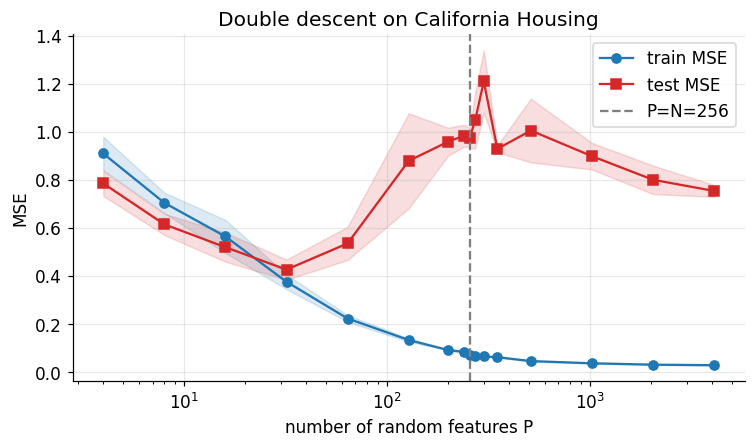
\includegraphics[width=0.75\linewidth]{double_descent.png}
  \caption{\textbf{Double descent on California Housing.} Test MSE (red) and training MSE (blue), mean $\pm$ standard deviation over three random-feature seeds, $\lambda = 10^{-3}$. The dashed gray line marks the interpolation threshold $P = N = 256$. The test-MSE peak at $P \approx 300$ is the double-descent spike.}
  \label{fig:doubledescent}
\end{figure}

\paragraph{Three-factor ablation.}
Figure~\ref{fig:three} reports the three ablations side by side. Each one flattens the spike.

\begin{figure}[t]
  \centering
  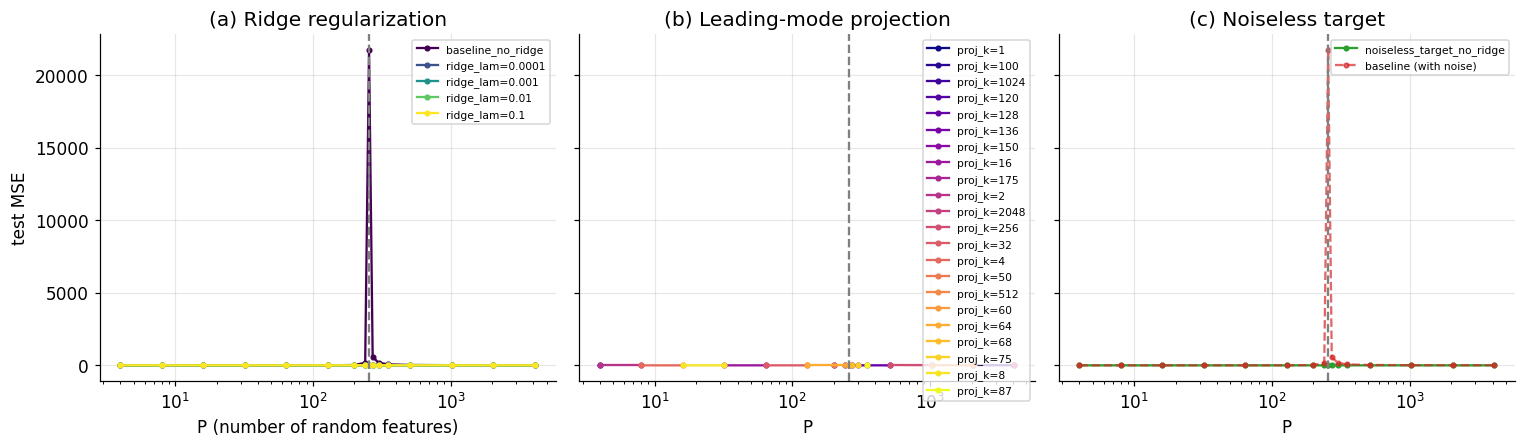
\includegraphics[width=\linewidth]{three_factor_ablation.png}
  \caption{\textbf{Three-factor ablation of double descent.} (a) Ridge sweep: increasing $\lambda$ progressively flattens the spike. The no-ridge baseline (lightest curve) blows up at $P = N$ due to numerical ill-conditioning. (b) Leading-mode projection: projecting test features onto the top $k = N/4$ or $k = N/2$ singular directions of $\Phi_{\text{train}}$ removes the spike. (c) Noiseless target: replacing $y$ with the best linear fit removes residuals and dampens the spike. Dashed gray line: $P = N$.}
  \label{fig:three}
\end{figure}

Table~\ref{tab:abl} reports test MSE at $P = N = 256$ for each ablation. The no-ridge baseline blows up to $\sim 2 \times 10^4$ because the smallest singular value of $\Phi_{\text{train}}$ is essentially zero at the interpolation threshold (next paragraph). Increasing $\lambda$ to $10^{-1}$ pulls test MSE down to $0.31$, projecting onto the top $N/4$ directions yields $0.35$, and the noiseless target with no ridge reaches $1.33$ (still better than the noisy baseline by four orders of magnitude). All three are consistent with the Schaeffer et al.\ account.

\begin{table}[t]
\centering
\caption{Test MSE at the interpolation threshold $P = N = 256$ under each ablation, mean over three feature seeds. Lower is better.}
\label{tab:abl}
\begin{tabular}{lc}
\toprule
Condition & Test MSE \\
\midrule
Baseline (no ridge) & $2.17 \times 10^4 \pm 2.66 \times 10^4$ \\
\midrule
(a) Ridge $\lambda = 10^{-4}$ & $3.15 \pm 0.35$ \\
(a) Ridge $\lambda = 10^{-3}$ (default) & $0.97 \pm 0.04$ \\
(a) Ridge $\lambda = 10^{-2}$ & $0.43 \pm 0.03$ \\
(a) Ridge $\lambda = 10^{-1}$ & $\mathbf{0.31 \pm 0.01}$ \\
\midrule
(b) Projection $k = N/2 = 128$ & $0.85 \pm 0.08$ \\
(b) Projection $k = N/4 = 64$ & $0.35 \pm 0.01$ \\
\midrule
(c) Noiseless target (no ridge) & $1.33 \pm 1.05$ \\
\bottomrule
\end{tabular}
\end{table}

\paragraph{Spectral collapse.}
Figure~\ref{fig:smallest} shows the smallest singular value of the random-feature matrix as a function of $P$. The value is $0.082$ at $P = 64$, drops to $0.0085$ at $P = 128$, plummets to $6.4 \times 10^{-7}$ at $P = N = 256$ (machine precision), and recovers to $\sim 0.0026$ at $P = 4096$. The dip is exactly at the interpolation threshold and is the structural witness for factor (a) of the Schaeffer account.

\begin{figure}[t]
  \centering
  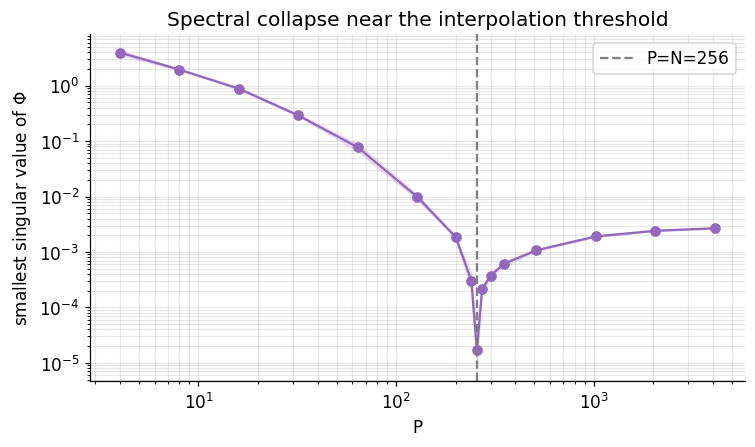
\includegraphics[width=0.75\linewidth]{smallest_singular_value.png}
  \caption{\textbf{Smallest singular value of $\Phi_{\text{train}}$ vs.\ $P$.} The smallest singular value collapses to near machine precision at $P = N$ (dashed gray) and recovers in the overparameterized regime. This is the structural quantity that ridge regularization stabilizes in factor (a).}
  \label{fig:smallest}
\end{figure}

\paragraph{Kernel approximation.}
Figure~\ref{fig:approx} compares random-feature ridge against the exact RBF kernel ridge baseline and against linear ridge. As $P$ grows, random-feature ridge approaches a plateau near the exact RBF kernel ridge value. On this dataset, however, both random-feature ridge and exact RBF kernel ridge are \emph{worse} than linear ridge ($0.55$). California Housing has strong linear structure and the RBF kernel is not a competitive choice for this data at the median-heuristic bandwidth. The convergence of random-feature ridge to exact RBF kernel ridge as $P \to \infty$ is still visible, which is the central kernel-approximation point. Whether the limiting kernel beats linear is a separate question of kernel choice.

\begin{figure}[t]
  \centering
  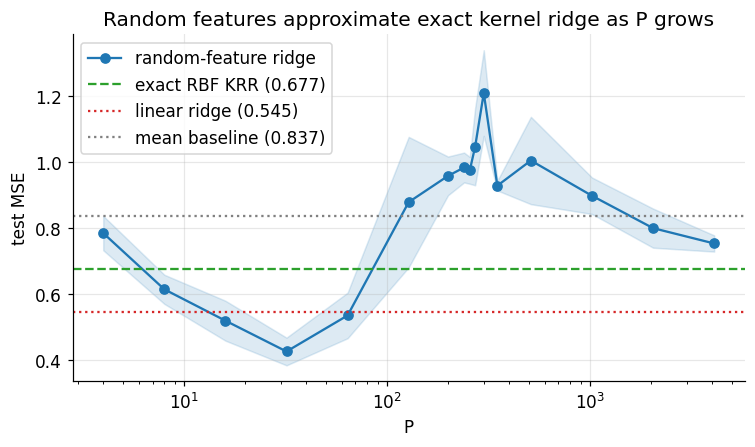
\includegraphics[width=0.75\linewidth]{kernel_approximation.png}
  \caption{\textbf{Random-feature ridge approaches exact RBF kernel ridge as $P \to \infty$.} Solid blue: random-feature ridge sweep with shading for seed standard deviation. Horizontal lines: exact RBF kernel ridge ($0.68$), linear ridge ($0.55$, the actual best on this dataset), and mean-predictor baseline ($0.84$). The double-descent spike is visible around $P = N$.}
  \label{fig:approx}
\end{figure}

\paragraph{Kernel-PCA spectrum.}
Figure~\ref{fig:kpca} shows the singular spectrum of the random feature matrix at varying $P$. At small $P$ the spectrum is short and decays slowly. As $P$ grows the spectrum lengthens, with leading singular values stabilizing and trailing singular values becoming progressively smaller. The spectrum near $P = N$ has a pronounced tail of near-zero singular values. In the overparameterized regime the bulk of the spectrum is preserved while the trailing tail recovers slightly.

\begin{figure}[t]
  \centering
  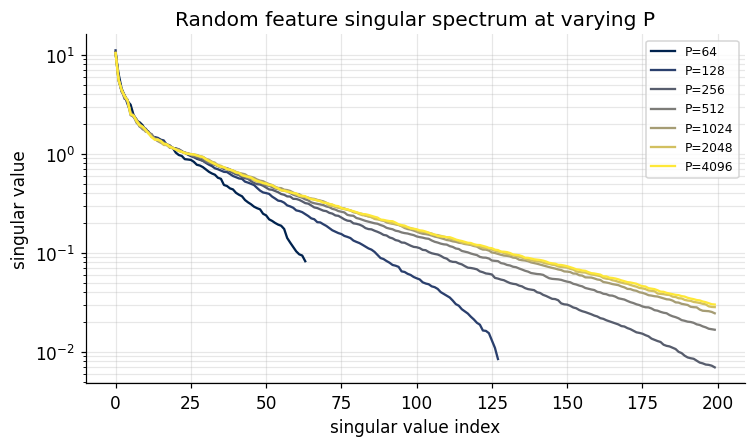
\includegraphics[width=0.7\linewidth]{kpca_spectrum.png}
  \caption{\textbf{Random-feature singular spectrum at varying $P$.} Each curve is the (descending-sorted) singular spectrum of $\Phi_{\text{train}}$ at one $P$ value, log scale. The spectrum lengthens as $P$ grows. Near $P = N$ the trailing tail drops to numerical zero, contributing the small-singular-value blowup that drives factor (a) of double descent.}
  \label{fig:kpca}
\end{figure}

\section{Discussion}

\paragraph{Putting the story together.}
Returning to the central question. Where does the classical bias-variance curve break, and what fixes it? It breaks because the ridgeless interpolator at $P = N$ is built on top of a near-singular feature matrix. The smallest singular value of $\Phi_{\text{train}}$ drops to machine precision exactly at $P = N$, the test MSE blows up to $\sim 2 \times 10^4$, and any of three independent fixes (ridge regularization, projection onto the leading singular directions, or a noiseless target) brings it back to near $0.3$. The geometry and the Schaeffer et al.\ account match.

\paragraph{All three factors are real, and any one is sufficient to flatten the spike.}
The Schaeffer et al.\ (2023) account predicts that ridge regularization, leading-mode projection, and noiseless targets are each sufficient to eliminate the test-error spike near $P = N$. Our results confirm this on California Housing. The most dramatic factor is ridge. Lifting $\lambda$ to $10^{-1}$ at the threshold reduces test MSE by four orders of magnitude, from a numerical-instability blowup to $0.31$. The most surprising factor in absolute terms is leading-mode projection. At $k = N/4$, test MSE at the threshold is $0.35$, matching the best ridge result without using $\lambda$ at all.

\paragraph{The geometry of the spike (smallest singular value).}
The smallest singular value of $\Phi_{\text{train}}$ drops to machine precision exactly at $P = N$ (Figure~\ref{fig:smallest}). The location of this dip matches the location of the test-MSE spike to within the resolution of our $P$ grid. This is the structural quantity that ridge stabilizes (factor a), that leading-mode projection sidesteps (factor b), and that has no error to amplify when targets are noiseless (factor c).

\paragraph{On the choice of dataset and kernel.}
California Housing is a standard tabular benchmark, but it has strong linear structure and the RBF kernel at the median-heuristic bandwidth does not outperform linear ridge. This affects the absolute scale of the kernel-approximation result but not the double-descent and three-factor results, which are about test-error \emph{shape} as $P$ varies, not about absolute predictive accuracy.

\paragraph{Limitations.}
We use a single dataset, a single kernel, and a small training subset ($N = 256$). The training subset size was chosen so the interpolation threshold could be cheaply spanned with our $P$ grid. The bandwidth was set by median heuristic and not separately tuned for predictive accuracy. Tuning it (or using a different kernel) could narrow the gap between random-feature ridge and linear ridge. The three-factor ablations remove the spike but do not separate the relative contribution of each factor. That would require factorial combinations of all three at once, which is beyond the scope of a single project.

\section{Conclusion}

We reproduced the double-descent test-error spike on California Housing using random Fourier feature ridge regression, and tested the three-factor explanation of double descent from Schaeffer et al.\ (2023) by ablating each factor in turn. Ridge regularization, leading-mode projection, and noiseless targets each eliminated the spike on their own. The smallest singular value of the random-feature matrix collapses to machine precision at $P = N$, providing the structural witness for the spike. Random-feature ridge approaches exact RBF kernel ridge regression as $P$ grows, although the RBF kernel itself is not the best choice for this dataset.

\paragraph{Reproducibility.}
All experiments use seed 42. Code is available at \href{https://github.com/nickvpn/vit-ml-xai-project}{github.com/nickvpn/vit-ml-xai-project} (project2 directory under \texttt{introml/}).

\begin{thebibliography}{12}

\bibitem{rahimi2007}
Rahimi, A.\ and Recht, B.\ (2007).
Random Features for Large-Scale Kernel Machines.
\textit{NeurIPS}.

\bibitem{belkin2019}
Belkin, M., Hsu, D., Ma, S., and Mandal, S.\ (2019).
Reconciling Modern Machine-Learning Practice and the Classical Bias-Variance Trade-off.
\textit{PNAS}, 116(32), 15849--15854.

\bibitem{schaeffer2023}
Schaeffer, R., et al.\ (2023).
Double Descent Demystified: Identifying, Interpreting and Ablating the Sources of a Deep Learning Puzzle.
\textit{arXiv:2303.14151}.

\bibitem{rasmussen2006}
Rasmussen, C.\ E.\ and Williams, C.\ K.\ I.\ (2006).
\textit{Gaussian Processes for Machine Learning}.
MIT Press.

\bibitem{scholkopf1998}
Sch\"olkopf, B., Smola, A., and M\"uller, K.\ (1998).
Nonlinear Component Analysis as a Kernel Eigenvalue Problem.
\textit{Neural Computation}, 10(5), 1299--1319.

\bibitem{hastie2022}
Hastie, T., Montanari, A., Rosset, S., and Tibshirani, R.\ (2022).
Surprises in High-Dimensional Ridgeless Least Squares Interpolation.
\textit{Annals of Statistics}, 50(2), 949--986.

\bibitem{bartlett2020}
Bartlett, P., Long, P., Lugosi, G., and Tsigler, A.\ (2020).
Benign Overfitting in Linear Regression.
\textit{PNAS}, 117(48), 30063--30070.

\bibitem{mei2022}
Mei, S.\ and Montanari, A.\ (2022).
The Generalization Error of Random Features Regression: Precise Asymptotics and the Double Descent Curve.
\textit{Communications on Pure and Applied Mathematics}, 75(4), 667--766.

\bibitem{pace1997}
Pace, R.\ K.\ and Barry, R.\ (1997).
Sparse Spatial Autoregressions.
\textit{Statistics \& Probability Letters}, 33(3), 291--297.

\bibitem{scikit-learn}
Pedregosa, F., et al.\ (2011).
Scikit-learn: Machine Learning in Python.
\textit{JMLR}, 12, 2825--2830.

\end{thebibliography}

\end{document}
